\chapter{Method} 
\label{chapter:Method}
\section{Singleton opinion spam detection}\label{section:singleton-detection}

The following section describes the experiments I have carried out in order to find the answers to two questions: can review spam be detected using a method based on semantic similarity? If so, how could semantic similarity be included in a complete method to detect singleton spam?

First, details on the structure and contents of the available review dataset are laid out. Following, the behavioral features used to cluster the reviews are explained in greater detail. Next, both the vectorial and semantic similarity measures are formulated along with examples of how they were applied. The clustering step is described afterwards. Finally, the opinion spam classifier validation step is explained together with a discussion about the performance metrics used to evaluate the results. 

The pseudocode on page \pageref{alg:singleton} shows all the steps of the detection method which are explained in this chapter.

\subsection{Dataset}

The Trustpilot dataset contains 8990 reviews written in English from 130 sellers, with an average of 70 reviews per seller. It is split in 4277 known fake reviews and 4713 truthful reviews. All the reviews have 4 and 5 stars and are from one-time reviewers, i.e. users that wrote a single review. They are collected from sellers which had at least 50 reviews. 

The fraction of filtered reviews out of all of the seller's reviews was set to be between 25\% and 75\%. The goal was to obtain a balanced dataset where each seller had both truthful and deceptive reviews and avoid sellers which had only truthful or only deceptive reviews. If a seller has had such a large percentage of reviews filtered out, it is even more likely the filtered reviews were indeed fake and that the remaining reviews are more trustworthy. 

For every review, the following information is available:
\begin{itemize}
\item review title
\item review text
\item review text length - the total number of characters in the text
\item review stars rating - either 4 or 5
\item review date
\item user sign up date - date when the user created his account on the review platform
\item seller identifier - a unique identifier for each seller
\item review IP - the IP from where the review was written. This has been obfuscated by dividing the long integer representation of the IP to a secret constant value, in order to obtain a real value in [0, 1]
\item proxy IP - boolean flag showing whether the specific IP collected when the review was created, has been identified as a proxy
\end{itemize}

\clearpage

\subsection{Data preprocessing}
From the raw data collected, I have designed several behavioral features and applied min-max normalization for all the reviews of each seller in order to obtain continuous values in [0, 1]. 

The min-max normalization is defined as:
\begin{equation}
x’ = \frac{x -min(x)}{max(x)-min(x)}
\end{equation}

\subsection{Behavioral features}
I have chosen to design the following features which will be used further on to cluster the reviews, separately for each seller:
\begin{description}
\item[IPRatio]: The long integer value of the IP is divided by the largest value this feature has from all the reviews in the dataset. In this way, two reviews made from the same IP will have the same feature value. The intention is to capture the similarity between IPs which differ only in the last octet, e.g. 88.123.45.2 and 88.123.45.107.
\item[IsProxy]: This binary feature is either 1 or 0 depending on whether the IP has been identified as being a proxy or not.
\item[UserSignedUpDateRatio]:  This is meant to capture the creation of multiple accounts in a short amount of time by a spammer. It is formulated as the ratio between the date when the user created his account, measured in date ticks and the oldest date that any user has signed up. This feature will have very similar values for users who create a range of accounts in a short time window.
\item[ReviewDateRatio]: This feature is the ratio between the date when the user wrote the review and the oldest date any user wrote a review. Its purpose is similar to that of the previous feature. If a user makes multiple reviews in a short amount of time, these reviews are very likely to end up in the same cluster.
\item[ReviewRating]: This feature represents the ratio between the stars rating of the review - 4 or 5, and the maximum rating - 5. Since the dataset contains only 4 and 5 stars reviews, the feature values will be 0.8 or 1. The intuition behind this feature is that a spammer is very likely to give the same high rating to the seller in multiple reviews. 
\item[ReviewTextLengthRatio]: This feature represents the number of characters in the review text. It is difficult for a spammer to make up a lot of lies about an buying experience he never had. So, it is likely he will reuse some content between multiple reviews and not alternate very much the length of his reviews. 
\end{description}

The main idea behind the engineered features is that users who create multiple accounts to post fake reviews for one seller usually do this in a short amount of time, give the same high rating and write about the same amount of characters in the review text. The designed features will be used further on in the clustering step, when reviews with similar feature values will end up in the same group. Clustering is required because as it will be explained in section \ref{subsection:clustering}, in practice, it is unfeasible to compare the text of any two reviews on a large review platform. 

Of course, the more features can be built from the dataset, the more efficient the grouping will be. It is a matter of how much information is available upfront. For example, new features could be built using details about the browser used by the users when posting reviews, such as the user agent information, location - country, city - or social network graph - in case the user preferred to authenticate through a social network.

\subsection{Review text preprocessing}

Several steps are needed in order to get the review text in a processable shape and to compute the vectorial and semantic similarity between reviews. First, I have used a part-of-speech tagger (or short POS tagger) to tokenize the reviews, remove stopwords and extract only some of the words for further processing. A POS tagger is a software system that given a piece of text in some language, can assign parts of speech (such as noun, verb, adjective, adverb, pronoun and so on) to the words in the text, \citet{StanfordNLPTagger}.
For this purpose, I have used the Stanford Log-linear Part-Of-Speech Tagger, described in more detail in \citet{Toutanova2003}.

Given for example the text:
\\*
\\*
\textit{I am working hard on my master thesis at DTU}
\\*
\\*The tagger first recognizes that there are 10 tokens in this text and outputs the following results:
\\*
\\*
\textit{I/PRP am/VBP working/VBG hard/RB on/IN my/PRP master/NN thesis/NN at/IN DTU/NNP}.
\\*
\\*
So, there are two verbs in the text: \textit{am} and \textit{working}, two pronouns \textit{I} and \textit{my}, two nouns - \textit{master} and \textit{thesis} and one proper noun - \textit{DTU}.

Besides POS annotations, the Stanford tagger is also capable of lemmatization, meaning that given a word, it can output its canonical, dictionary form, e.g. for the word \textit{am}, it can output its lemma \textit{be}. Or for \textit{working}, it outputs \textit{work}. 

Besides the verbs, nouns, adjectives, adverbs and pronouns, sentences contain many other connecting words that add a small amount of semantic value. Words such as \textit{a}, \textit{to}, \textit{be}, \textit{or}, \textit{any}, \textit{among} provide little context by themselves and are usually removed from the text in the preprocessing step. The reason is that they are more frequent than the useful words that actually provide most of the information. Due to their frequency, they can influence the similarity value between sentences. They can make two sentences be considered more similar than they actually are, just because both contain many stopwords. 

The final preprocessing step is removing the stopwords from all the reviews and for this purpose, I have used a stopwords list created by Gerard Salton and Chris Buckley for the experimental SMART information retrieval system at Cornell University. It is considered more "aggressive" than other freely available lists as it contains more items, \citet{SaltonandBuckleyStopWordsAggresive}.

\subsection{Similarity measures}
My goal was to test the hypothesis that semantic similarity generally outperforms vectorial-based measures for opinion spam detection and when that is not the case, to propose a similarity measure based on a combination of vectorial and semantic measures that performs better than each taken separately. More concretely, I have compared the results of three variants of the cosine similarity and the semantic similarity measure of \citet{Mihalcea2006}, when computing the similarity of review pairs. 

I have experimented with different combinations of parts-of-speech among nouns, verbs, adjectives, adverbs and pronouns. All of the POS sets included at least nouns and verbs because these words contain most of the information in a sentence and the semantic similarity measure which relies on the WordNet database works best on this type of words. Then I verified if adding the other POSs one by one and all together actually improves the model.

Following, I will try to explain the underlying implementation of my model, through a simple example - taking two extremely short review texts as examples and going through all the semantic similarity measures I have applied. In the available dataset from Trustpilot, reviews are longer than the ones in this example.
Given two very short reviews written by two different users:
\\*
\\*
\textit{I had a issue once that took a bit to fix but other then that its a great site.}
\\*
\\*
\textit{My first order with them didn't go through because of some site issues.}
\\*
\\*
When reading the two reviews, it is obvious both users had some issue with the seller. After tokenizing the two texts, the extracted words are:
\\*
\\*
\textit{I, had, a, issue, once, that, took, a, bit, to, fix, but, other, then, that, its, a, great, site}
\\*
\\*
\textit{My, first, order, with, them, didn, t, go, through, because, of, some, site, issues}

\subsubsection{Cosine similarity}
(all words, excluding stopwords)

For this method, I have considered all words in the reviews and only eliminated stopwords, meaning all the words that appeared in the list of \citet{SaltonandBuckleyStopWordsAggresive}.
This measure is very easy to implement in a production system, because it consists of splitting a text into words by removing spaces and basic punctuation marks, such as ".", "!", "?". The two sets of words from each document are then joined, resulting in two document vectors containing the number of occurrences of each word in each document. Comparing the two vectors is a cheap operation by today's hardware standards.

It can be observed that first of all not removing the stopwords would have some negative implications on the similarity result. The most frequent word in the first text is the article "a" which is repeated 3 times, although it does not offer any useful contextual information about what the text might be about. Also, the word "that" which is mentioned twice does not contribute much to the meaning of the text. 
\\*
\\*
\textit{I, had, \textbf{a}, issue, once, \textbf{that}, took, \textbf{a}, bit, to, fix}
\textit{but, other, then, \textbf{that}, its, \textbf{a}, great, site}
\\*
\\*
Joining the two sets of extracted words after excluding the stopwords results in the following set:
\\*
\\*
\textit{issue,bit,fix,great,site,order,didn}
\\*
\\*
The bag of words representations for the two texts are the following vectors:

[1,1,1,1,1,0,0]

[1,0,0,0,1,1,1]

Computing the cosine similarity of the two vectors outputs a score of 0.44, which is much higher than what the cosine would have scored if the stopwords had not been removed - only 0.05.

\subsubsection{Cosine similarity with non-lemmatized POSs}
(nouns/verbs/adjectives/adverbs/pronouns only, excluding stopwords)

For these experiments, I have used the Stanford Log-linear Part-Of-Speech \citet{StanfordNLPTagger} to tokenize the texts and extract only the nouns, verbs, adjectives, adverbs and pronouns. Also, I eliminated all the words that appeared in the stopwords list of \citet{SaltonandBuckleyStopWordsAggresive}. 
The results for the two short texts used in the previous example were the following:
\\*
\\*
\textit{issue, bit, fix, great, \textbf{site}}
\\*
\\*
\textit{order, n’t, \textbf{site}, issues}
\\*
\\*
As it can be seen, the number of words has been considerably reduced to a set of words that capture most of the meaning of the texts and the stopwords no longer have an impact on the two underlying vectors.
The joined extracted words from the two texts results in the following set:
\\*
\\*
\textit{issue,bit,fix,great,site,order,n't,issues}
\\*
\\*
The vectorial representations for the two texts becomes [1,1,1,1,1,0,0,0] and [0,0,0,0,1,1,1,1]. 

Computing the cosine similarity of the two vectors outputs a score of 0.22. This shows very good improvement over the previous raw cosine measure but the disadvantage is that this approach takes a performance hit when the texts are tokenized through the POS tagger. Fortunately, the Stanford tagger performs very fast and these two texts are also very small, so the slowdown is not noticeable. However, it would become noticeable for example when tagging all the reviews from a seller that has 50,000 regular-sized reviews.

Furthermore, I have experimented with different sets of POSs, such as only nouns, verbs, adjectives and adverbs, or only nouns, verbs and adjectives. In this last case example, since "not" is an adverb, it is excluded and the overall similarity score rises to 0.25.
Still, it is obvious the similarity score could be improved further if the words "issue" and "issues" would be represented as the same word in the two vectors and this will be presented next. 

\subsubsection{Cosine similarity with lemmatized POSs}

(nouns/verbs/adjectives/adverbs/pronouns only, excluding stopwords)

POS tagging and stopwords removal has helped to outperform the raw cosine similarity, but comparing only the words roots would improve the similarity even more. In order to compute this new cosine-based measure, I have used the lemmatization feature from the Stanford tagger, so instead of building the vectors using the raw words, I have replaced all the words with their lemmas. 

The results for the two short texts used in the previous example now become:
\\*
\\*
\textit{\textbf{issue}, bit, fix, great, \textbf{site}}
\\*
\\*
\textit{order, not, \textbf{site}, \textbf{issue}}
\\*
\\*
Joining the two results in the following set:
\\*
\\*
\textit{issue,bit,fix,great,site,order,not}
\\*
\\*
The cosine similarity of the two vectors [1,1,1,1,1,0,0] and [1,0,0,0,1,1,1] now rises to 0.45. 
This shows lemmatization considerably improves the similarity score of two texts by "flattening" out the words to their dictionary roots. However, this does not capture any semantic relationship between the two texts. 

The first review could have very well have said:

\clearpage

\textit{I had a problem one time with an order and it took a bit to fix, otherwise this is an awesome website}, 
\\*
\\*
while the second review could have said: 
\\*
\\*
\textit{My first order with them didn't go through because of some site issues, but all in all this is a great website}.
\\*
\\* 
The cosine similarity with lemmatized POSs goes down to 0.33 because some of the words have been changed with synonyms. A human reading these two texts would immediately see the two reviews talk about the same things. The semantic similarity presented next outputs a similarity score of 0.5, capturing more similarities than the cosine-based methods.

\subsubsection{Semantic similarity from \citet{Mihalcea2006}}

In order to compute the semantic similarity between reviews, I have used the Semilar toolkit developed by \citet{Rus2013}. The toolkit aims to offer a unified environment for researchers and developers to easily access many semantic methods for word-to-word, sentence-to-sentence and document-to-document similarity, as described by \citet{SEMILAR}.

The Semilar toolkit is available as a Java library. I have used C\# to write the implementation for this project. In order to integrate and be able to use it from my code, I have used the IKVM.NET tool to create a .NET consumable assembly out of the Java library. IKVM is basically a Java Virtual Machine implemented in .NET including a .NET implementation of Java class libraries, which aims for Java-.NET interoperability \citet{IKVMNET}. 
At this point, I was able to load any two reviews from the dataset, feed the pair into the Semilar toolkit and get the semantic similarity results using all the available methods. I have run several experiments using real-life reviews from my dataset where I tried to compare results obtained with other semantic similarity measures included in the toolkit, such as Leacock \& Chodorow, Lesk, Wu \& Palmer, Resnik, Lin, and Jiang \& Conrath. Mihalcea’s measure, as it is also stated in her paper, proved superior to all, so I will not mention these other results.

As it will be seen in the results section, the semantic similarity measure of \citet{Mihalcea2006} has outperformed the cosine-based measures. In the simplistic example of the two reviews where the lemmatized parts-of-speech variant of the cosine similarity topped 0.45, the semantic similarity value scored 0.48. In the modified example where some of the reviews’ words were replaced by close synonyms, the cosine topped at 0.33, while the semantic measure went up to 0.5. As the results section will show, this difference increases when testing on real-life reviews with more words.

Several improvements could be made to the semantic measure, such as computing the \textit{idf} for my review corpus. These values have already been computed using a different corpus in the Semilar toolkit. 

Since WordNet gives very good results when used for word-to-word comparisons, extending the measure to sentence-to-sentence and document-to-document levels should involve more contextual information. In the toolkit, this case is handled in two ways: either the most frequent sense of a word is always used, either for all the senses of a word, the maximum or average of the relatedness score from WordNet is used, \citet{Rus2013}.
I have not been able to find where to configure this switch between the two strategies since the authors behind the toolkit are yet to release more extensive documentation. So I am not sure which of the two strategies is being used by default or if the best results of the two is considered.

\subsubsection{\textit{Maxsim} - maximum value from all the previous measures}

The purpose of this new proposed similarity measure is to try and make the best of both worlds - vectorial and semantic. Although intuitively, the semantic similarity should always outperform the vectorial counterpart since every word should be semantically identical first of all to itself, the results will show that there are times when the cosine similarity gives better precision in relation to the classifier validation techniques used. So, perhaps choosing the maximum value from all vectorial and semantic measures for any pair of reviews should always achieve the highest precision.

\clearpage

\subsection{Clustering}\label{subsection:clustering}
The next step is to create clusters of reviews using the defined behavioral features. Clustering is needed to reduce the singleton opinion spam algorithm running time. Practically it is unfeasible to compare the text of any two reviews for any seller on a large review platform. Comparing each review with all the rest would mean a number of operations close to n\textsuperscript{2}/2, which has a complexity of O(n\textsuperscript{2}). Given a seller which has 20,000 reviews and assume a very optimistic speed of only 100 milliseconds for doing all of the following: removing stopwords, parts-of-speech tagging, looking up a word senses in WordNet, computing a relatedness score for each word pair, then computing the Mihalcea formula for all the words in the review pair. Roughly, it would take about half a year to compare all the reviews, so it is obvious this strategy could not work.

There are several strategies to perform clustering, but looking from a simplistic perspective there are only two. The first one assumes the target number of clusters is known upfront and all we are after is a reasonable split of the data to match this input number (K-means). The second type is helpful if this target is not known upfront and the items need to be grouped with the help of a distance metric that expresses the connectivity between the various data objects.

Since I did not know the number of review clusters ahead, I decided that a density-reachability clustering technique would intuitively apply well to my data, because of the way spammers create fake reviews. They usually give the same high rating and post reviews in dense bursts, in a relatively short amount of time. This assumption has been proven by many studies presented in the \nameref{chapter:relatedwork} chapter. 

I have used two popular data mining frameworks that include many clustering algorithms: ELKI and Weka, both open source projects and both written in Java. They are both aimed at researchers and academics. Weka (\citet{WEKA}) is more or less the de facto machine learning toolkit for academia students, has a nice user interface and provides good visualizations. ELKI (\citet{ELKI}) prides itself with having the best performing implementations for clustering and outliers detection algorithms. Also, it provides a well documented benchmark for performance of the density based clustering algorithms compared to Weka and it claims that Weka cannot even run some of the clustering algorithms on large datasets in acceptable time. I was able to confirm this benchmark by running the same clustering algorithms on ELKI and Weka using my dataset. In the end, I decided to go with ELKI and tried out two density based clustering algorithms - DBSCAN and OPTICS.

The Density-based spatial clustering of applications with noise (DBSCAN) algorithm has been proposed by \citet{Ester96} and is based on the notion of density reachability. Simply put, a data point \textit{p} is reachable from a point \textit{q} if the distance from \textit{p} to \textit{q} is below a fixed threshold epsilon. The formed clusters have a very useful property, that any data point that is density-connected to any data point inside a cluster will become part of that cluster also. 

The algorithm requires two parameters: \textit{minPts} and \textit{epsilon}. The first represents the minimum number of points in a cluster, while \textit{epsilon} is the maximum "jump" distance from one point to another point, which will end up in the same cluster as the first point if the condition is satisfied. Figure \ref{dbscan} shows B and C are density-connected to A, thus all three points, A, B and C will be in the same cluster, \citet{DBSCAN-Illustration}.

\begin{figure}[ht!]
\centering
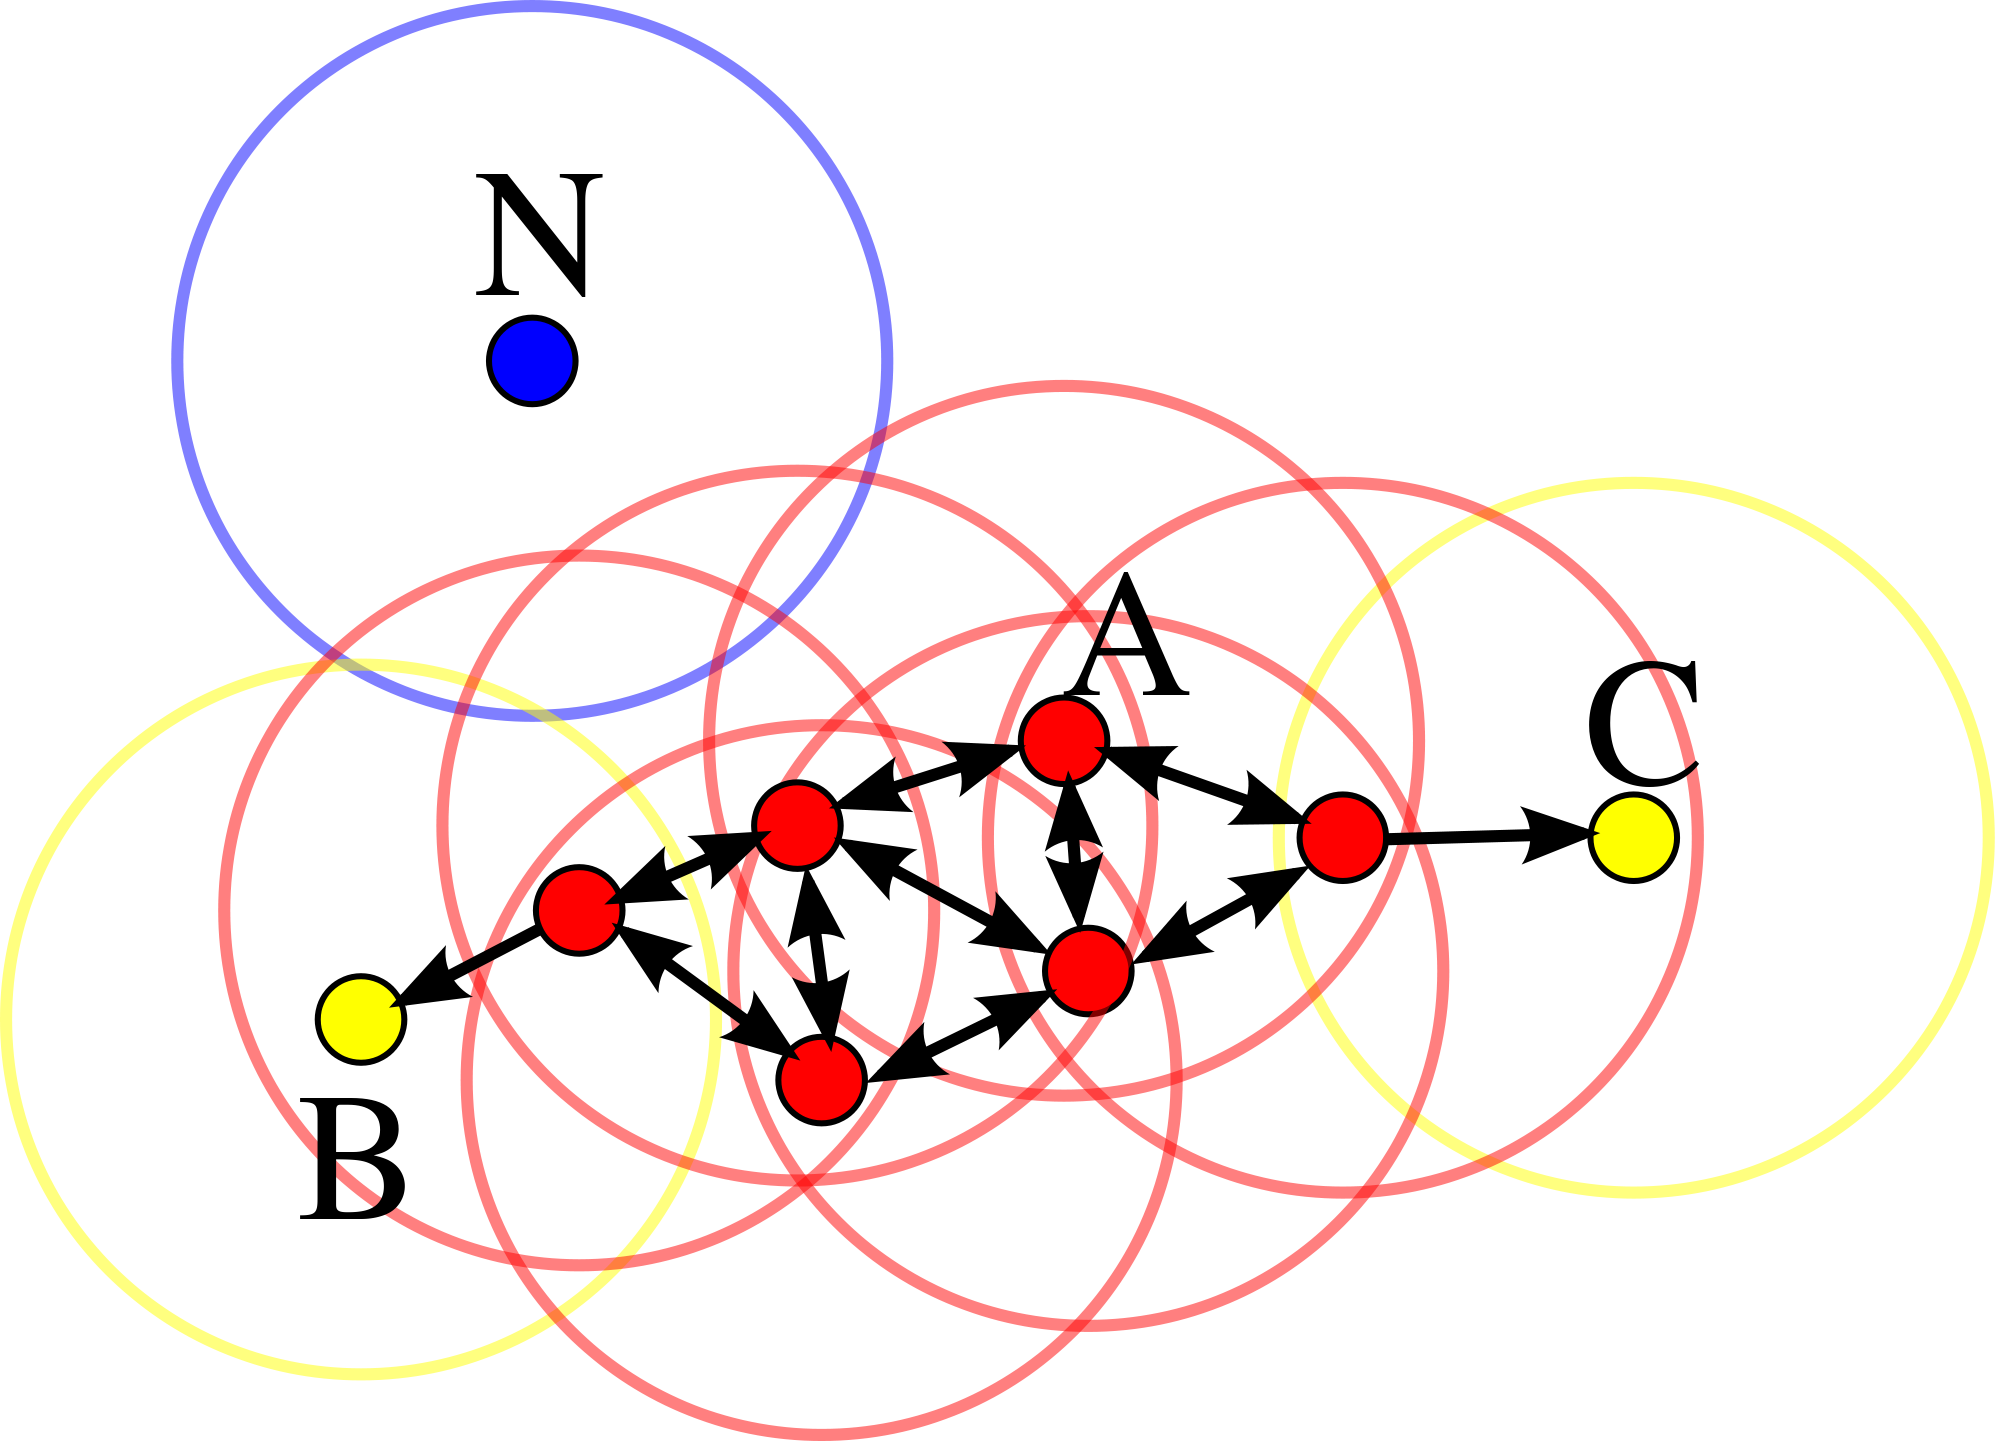
\includegraphics[width=7cm,height=5cm,keepaspectratio]{figures/dbscan.png}
\caption{DBSCAN illustration}
\label{dbscan}
\end{figure}

This property makes DBSCAN suitable for the opinion spam detection problem since it should keep the deceptive reviews written by the same spammer grouped in the same cluster. The reviews written by a spammer can be distributed over several days and this chaining property is implicitly modeled by the algorithm. 

DBSCAN also captures noise - the data points which do not satisfy the \textit{epsilon} threshold in relation to their distance from another point already in a cluster, do not end up in any cluster.

I have experimented with minimum 2 and 3 points per cluster, i.e. \textit{minPts} in \{2, 3\}. 
Since I have normalized all the features to have values in [0, 1], I experimented with \textit{epsilon} in \{0.01, 0.05, 0.08, 0.1, 0.4\}. This way I could also choose the most convenient \textit{epsilon} value that hits the right balance between cluster size and noise. 

A high \textit{epsilon} would create large review clusters - e.g. sellers which recently signed up to the review platform and received hundreds of 5 star reviews in a very short amount of time. The clustering noise in this case would be very small, because most of the reviews would end up in a cluster, but this is exactly the problem clustering is supposed to help fix. A low \textit{epsilon} would create small and really good quality compact clusters in terms of reviews being posted very close to each other, with exactly the same ratings, from similar IPs and so on. But this would also generate a lot of noise - reviews which are outside of any cluster. In practice, for small values of \textit{epsilon} as it will be seen in the results section, only 20\% of the reviews were actually clustered. This is not very useful in real-life scenarios and the purpose is to find just the right balance for \textit{epsilon}.

It is known that DBSCAN does not work well with high dimensional data but this is not the case in the review dataset I have used. Also since \textit{epsilon} value is fixed upfront, it does not detect meaningful clusters of variable densities. The basic idea behind the Ordering Points To Identify the Clustering Structure (OPTICS) algorithm is the same as DBSCAN’s, but this can handle the variable density clustering much better. No \textit{epsilon} value is required, the only input is the minimum number of data points any cluster should contain. 

The Trustpilot dataset contains reviews from multiple sellers and the spam patterns associated with each seller should intuitively be different from one another. Spammers posting fake reviews on one seller’s company page cheat differently than spammers working for another seller: the first may all use known proxies and post reviews very close to each other, while the second group may use obscure undetected VPNs and post reviews over a longer period of two weeks for example.

I have run two clustering experiments to see which algorithm performs best on my dataset and adjusts better to these types of user behavior. For DBSCAN, I have chosen \textit{epsilon} in \{0.01, 0.05, 0.08, 0.1, 0.4\} and experimented with each value for all sellers. Since OPTICS figures out the epsilon value by itself, it should end up with a different value for each seller and possibly come up with clusters which better capture the users behavior per seller than DBSCAN. 

For each cluster obtained, I have computed the following text similarity measures among each pair of reviews:
\begin{itemize}
\item cosine similarity with all words, excluding stopwords
\item cosine similarity with only non-lemmatized POS - combinations between nouns, verbs, adjectives, adverbs and pronouns, excluding stopwords
\item cosine similarity with only lemmatized POS - combinations between nouns, verbs, adjectives, adverbs and pronouns, excluding stopwords
\item mihalcea semantic similarity - combinations between nouns, verbs, adjectives, adverbs and pronouns, excluding stopwords
\item maximum value among of all the previous measures
\end{itemize}

I have considered different combinations of POSs including at least nouns and verbs, then adding each or all of adjectives, adverbs and pronouns, in order to see which of them give better results.
Finally, for every cluster I computed the maximum value of each of the 5 measures for all pairs of reviews in the cluster. 

Given two reviews $R_i$ and $R_j$ from a cluster C and a similarity measure chosen from the 5 ones above, the maximum similarity value is defined below as:
\begin{equation}
MaxSimilarity = \max\limits_{R_i, R_j\in{C}}(similarity\_measure(R_i, R_j))
\end{equation}

\subsection{Classifier output validation}\label{subsection:validating_classifier_output}

The results from each of the similarity measures are real values in [0, 1]. In order to separate truthful reviews from deceptive ones, I have defined a spam threshold, also a real number in [0, 1] which works in the following simple way: if the similarity value is lower than the threshold, the reviews are classified as truthful, otherwise they are deceptive. Intuitively, as the threshold is increased, the better the classifier should work in terms of precision. 

Next, I have applied two strategies to validate the classifier's output:
\begin{description}
\item[Cluster strategy] - if the maximum similarity recorded between any two reviews inside each cluster was above the threshold, then all the reviews in the cluster were considered deceptive, otherwise they would be considered truthful.
\item[Individual review pair strategy] - this was also applied inside each cluster, such that if the similarity measure between any two reviews from the same cluster was above the threshold, then only the two reviews would be considered deceptive, otherwise both would be considered truthful.
\end{description}

The first strategy acts as a coarse-grained mechanism penalizing all the reviews in the cluster if any of the contained pairs scores a similarity above the threshold. So, users get penalized just by being in the close vicinity of highly suspicious users, by sharing the same cluster. Intuitively, this approach should give a lower precision than the individual review pair strategy, but a higher recall. 

On the other hand, the individual review pair strategy should achieve the best precision because of its fine granularity. A more general mitigation approach could automatically filter out the review pairs scoring above the threshold and then consider the rest of their cluster neighbors as highly suspicious reviews, but apply more detection methods or manual validation before making a final decision to mark them as truthful or as deceptive. 

\subsection{Performance metrics}

The problem of detecting opinion spam can be treated as a binary classification task: given a dataset of reviews, the goal is to divide it into two sets of truthful and deceptive reviews. One popular method for computing the performance of a binomial classifier is by using precision, recall and the combination of the two into a single value - the F1 score.

Out of all the reviews classified as deceptive, only a fraction \textit{p} is indeed deceptive and this is defined as precision. And from the total number of deceptive reviews in the dataset, the classifier can detect a fraction \textit{r} and this is known as the classifier’s recall. 
\begin{equation}
precision = \frac{tp}{tp + fp}
\end{equation}
\begin{equation}
recall = \frac{tp}{tp + fn} 
\end{equation}, where
\begin{description}
\item[tp] = true positives, number of reviews classified as deceptive which were indeed deceptive
\item[fp] = false positives, number of reviews classified as deceptive which were actually truthful
\item[tn] = true negatives, number of reviews classified as truthful which were indeed truthful
\item[fn] = false negatives, number of reviews classified as truthful which were actually deceptive
\end{description}

The F1 score is defined as the harmonic mean between precision and recall as:
\begin{equation}
F1Score =  2\cdot\frac{precision*recall}{precision+recall}
\end{equation}

There is always a trade-off between the precision and recall, because in practice it is extremely hard to tune the classifier so that both are as close to 1 as possible. It really depends on the problem at hand and most of the time a decision is made to aim for a really good value of one of the measures. In my case, precision is critical, because it is more important to avoid filtering out truthful reviews by mistake than not to catch all the spammers. 
Since I have tested multiple similarity methods between reviews, it is important to be able to say which one is actually the best at detecting fake reviews. And since the classifier performance is shown by two measures, I have used the F1 score to combine the two into a single value and then more easily choose the similarity method which performs best. 

The pseudocode below summarizes all the method's steps.

\begin{algorithm}[!ht]
\caption*{Pseudocode for the singleton opinion spam detection method}
\label{alg:singleton}
\begin{algorithmic}[1]
\For{each review $R$ in dataset}
	\State Remove stopwords
  	\State Extract POSs
  	\EndFor
  	\State Cluster reviews using the behavioral features
  	\For{each cluster $C$}
  		\For{each reviews pair ($R_i$, $R_j$) $\in$ $C$}
		\State $\underset{R_i, R_j \in C}{sim}(R_i, R_j)$ = $\underset{R_i, R_j \in C}{similarity\_measure}(R_i, R_j)$
	\newline\Comment{${similarity\_measure}$ is each measure out of \{cosine, cosine pos non lemmatized, cosine pos lemmatized, mihalcea and maxsim\}}
		\EndFor
		\State ${sim(C)}$ = $\underset{R_i, R_j\in C}{\max(sim(R_i, R_j))}$
		\For{$spam\ threshold\ T = 0.5$, $T <= 1$, $T{+=}{0.05}$}
			\newline\Comment{cluster validation strategy}
			\If{${sim(C)}$ > ${T}$} 		
				\State Mark all reviews in cluster $C$ as deceptive
			\Else 
				\State Mark all reviews in cluster $C$ as truthful
			\EndIf
			\newline\Comment{individual review pair validation strategy}
			\If{${sim(R_i, R_j)}$ > ${T}$}
				\State Mark $R_i$ and $R_j$ as deceptive
			\Else 
				\State Mark $R_i$ and $R_j$ as truthful
			\EndIf
		\EndFor
	\EndFor
\end{algorithmic}
\end{algorithm}

\clearpage 

\section{Distribution of truthful and deceptive reviews}\label{section:distribution-reviews}

The purpose of this experiment was to find out if there is a distributional difference, for both vectorial and semantic similarity measures, between deceptive and truthful reviews inside the Trustpilot dataset as well as in the well known dataset used by \citet{Ott2011}. Recall that Ott obtained deceptive reviews using Amazon Mechanical Turk - the turkers had to imagine staying at the specific hotels and write their reviews to sound as credible as possible. 

\citet{Mukherjee2013a} made an interesting observation in their study: the spammers caught by Yelp's filter seem to have "overdone faking" in their attempt to sound more genuine. In their deceptive reviews, they used words that appeared in genuine reviews almost equally frequent and avoided to reuse the exact same words over and over again in their deceptive reviews. This is exactly the reason why a cosine similarity measure is not enough to catch subtle spammers in real life scenarios, such as Yelp's. 

The cumulative distribution function (CDF) can show this aspect which is more likely to appear when computing semantic similarity between reviews. The CDF gives the probability of a random variable \textit{X}, which has a known probability distribution, to have a value less or equal to \textit{x}, as shown in the definition below.
\begin{equation}
CDF_X(x) = \operatorname{P}(X\leq x).
\end{equation}

The purpose of the CDF curves of truthful/fake reviews is to check if they overlap or there is a separation margin between the two curves. If indeed there is a gap, it would be interesting to know how big this separation is and what are its bounds. 

First of all, the 800 reviews (400 truthful and 400 deceptive) from the \citet{Ott2011} dataset have been preprocessed. I have used the Stanford Log-linear Part-Of-Speech \citet{StanfordNLPTagger} to tokenize the texts and extract only the nouns, verbs and adjectives from each review. Also, I eliminated all the words that appeared in the stopwords list of \citet{SaltonandBuckleyStopWordsAggresive}. Next for each review pair in both separate subsets of truthful/deceptive reviews, I have computed their vectorial similarity, i.e. cosine, cosine without lemmatization and cosine with lemmatization, and their semantic similarity, i.e. the method from \citet{Mihalcea2006}. The same steps were applied also to the Trustpilot dataset.

The results have been plotted and discussed in the \nameref{chapter:Results} chapter.

\clearpage

\section{Aspect-based mining for opinion spam detection}\label{section:aspect-mining}

Topic modeling and in particular Latent Dirichlet Allocation (LDA) have been proven to work very well to extract aspects from user reviews. LDA is described more formally in Figure \ref{fig:lda-graphical-model},

\begin{figure}[htp]
  \centering
  \begin{tikzpicture}
    [
      observed/.style={minimum size=15pt,circle,draw=blue!50,fill=blue!20},
      unobserved/.style={minimum size=15pt,circle,draw},
      hyper/.style={minimum size=1pt,circle,fill=black},
      post/.style={->,>=stealth',semithick},
    ]

    \node (w-j) [observed] at (0,0) {$w_{d,n}$};
    \node (z-j) [unobserved] at (-1.5,0) {$z_{d,n}$};
    \node (z-prior) [unobserved] at (-3,0) {$\theta_d$};
    \node (z-hyper) [label=above:$\alpha$] at (-4.5,0) {};
    \filldraw [black] (-4.5,0) circle (3pt);
    \node (w-hyper) [label=above:$\beta$] at (-1.5,1.5) {};
    \filldraw [black] (-1.5,1.5) circle (3pt);
    
    \path
    (z-j) edge [post] (w-j)
    
    (z-hyper) edge [post] (z-prior)
    (z-prior) edge [post] (z-j)

    (w-hyper) edge [post] (w-j)
    ;

    \node [draw,fit=(w-j) (z-prior), inner sep=14pt] (plate-context) {};
    \node [above right] at (plate-context.south west) {$D$};
    \node [draw,fit=(w-j) (z-j), inner sep=10pt] (plate-token) {};
    \node [above right] at (plate-token.south west) {$N$};

  \end{tikzpicture}
  \caption{Plate Diagram of LDA. For more information, see \citet{Blei:2003:LDA:944919.944937} }
  \label{fig:lda-graphical-model}
\end{figure}

where
\\{$\theta_d$} represents the topic proportions for the \textit{d}th document
\\{$z_{d,n}$} represents the topic assignments for the \textit{n}th word in the \textit{d}th document
\\{$w_{d,n}$} represents the observed word for the \textit{n}th word in the \textit{d}th document
\\{$\beta$} represents a distribution over the words in the known vocabulary

I have considered the LDA topics to be equivalent to the aspects extracted from the reviews. Under this perspective, I have tried to test the hypothesis that reviews created by the same persons using multiple accounts would have similar topic distributions. 

\subsection{Data preprocessing}

For these experiments, I have used the Trustpilot labeled dataset containing 8990 reviews split almost equally between known truthful and deceptive reviews. Similar to the initial experiments, first, I eliminated all the stopwords that appear in the list created by  \citet{SaltonandBuckleyStopWordsAggresive}, then I have used the Stanford Log-linear Part-Of-Speech Tagger \citet{StanfordNLPTagger} to tokenize the reviews and extract only the nouns, verbs and adjectives. After these steps, I computed the frequency of the words in the new corpus and plotted the frequency histogram to check the distribution of the remaining words. The goal was to remove more uninformative, highly seller-specific words, i.e. words with very low frequency, as well as highly frequent words, such as for example \textit{buy}, \text{price} and \textit{service} which occurred more than 2000 times in the 9000 reviews. These words are inducing noise into the topic distribution and could be added to the stopwords list from the initial preprocessing step. Figure \ref{fig:lda-words-hist} in the \nameref{chapter:Results} chapter shows the words distribution before and after the removal of the extra frequent words. 

Furthermore, reviews which did not have at least 10 words after the previous words filtering step were also removed from the corpus, since the quality of the LDA topics is known to be low for short and sparse texts. There were many reviews which after the initial word-frequency filtering ended up having a single word. Each word comes from exactly one topic in LDA, so for one-word documents, it means that one topic would have a very high weight and the other topics would have very low weights. Thus when paired with other reviews, the similarity score would be very low. 

\subsection{Similarity measures}

Each review is a distribution over topics, so computing the similarity between two reviews translates to computing the similarity between their underlying topic distributions. The Kullback-Leibner (KL) \citet{Kullback1951} measures the difference between two probability distributions \textit{P} and \textit{Q} as shown in equation \ref{eq:KL}. So it can be used to compute a value for the distance between the underlying topics distributions of two reviews. This measure has two drawbacks though. If \textit{Q(i)} is zero, then the measure is undefined. It is also not symmetric, meaning the divergence from \textit{P} to \textit{Q} is not the same as that from \textit{Q} to \textit{P}. Translating this to the reviews context, it is not a suitable metric to use, because if a review \textit{$R_1$} is similar to \textit{$R_2$} then it would be expected that \textit{$R_2$} is similar with the same amount to \textit{$R_1$}.

\begin{equation}\label{eq:KL}
KL(P\|Q) = \sum_i \ln\left(\frac{P(i)}{Q(i)}\right) P(i).\!
\end{equation}

The Jensen-Shannon (JS) measure is based on the KL divergence and it addresses these drawbacks: it is symmetric and always provides a finite value. It is also bounded by 1, which is more useful when comparing a similarity value for a review pair with a fixed threshold in order to classify the reviews as fake. Equation \ref{eq:JS} formulates the JS measure.

\begin{equation}\label{eq:JS}
JS(P \parallel Q)= \frac{1}{2}KL(P \parallel M)+\frac{1}{2}KL(Q \parallel M), \hspace{0.2cm} where \hspace{0.2cm} M=\frac{1}{2}(P+Q)
\end{equation}

The JS measure can be rewritten in the form of equation \ref{eq:IR}, in order to decrease computational time for large vocabularies, as mentioned by \citet{dagan1999similarity}. IR is short for information radius, while {$\beta$} is 
a statistical control parameter.

\begin{equation}\label{eq:IR}
IR(P,Q) = 10^{-\beta{JS(P \parallel Q)}}
\end{equation}

The IR measure was applied to all review pairs forming the new corpus, after the data preprocessing step. Similar to the model presented in section \ref{section:singleton-detection}, similarity thresholds were used to validate the output from the review classifier. The validation procedure was the individual review pair strategy presented earlier in section \ref{subsection:validating_classifier_output}, with the small change that instead of applying it to clusters, it was applied to all the reviews from a seller. The computed similarity was then compared to a fixed spam threshold in order to predict whether the reviews were truthful or deceptive. 

The pseudocode above summarizes the method's steps.
\begin{algorithm}
\caption*{Pseudocode for the aspect-based mining for opinion spam detection method}
\label{alg:aspect-mining}
\begin{algorithmic}[1]
	\For{each review $R$ in dataset}
		\State Remove stopwords
	  	\State Extract nouns, verbs and adjectives
  	\EndFor
  	\State Run LDA for \#topics {$\in$} \{10, 30, 50, 70, 100\}
	\For{each \#topics}
	  	\For{each reviews pair ($R_i$, $R_j$)}
		\State $sim(R_i, R_j)$ = $\underset{R_i{\sim}T_i, R_j{\sim}T_j}{similarity\_measure}(T_i, T_j)$
		\EndFor
		\For{$spam\ threshold\ T = 0.5$, $T <= 1$, $T{+=}{0.05}$}
			\If{${sim(R_i, R_j)}$ > ${T}$}
				\State Mark $R_i$ and $R_j$ as deceptive
			\Else 
				\State Mark $R_i$ and $R_j$ as truthful
			\EndIf
		\EndFor
	\EndFor
\end{algorithmic}
\end{algorithm}

I have used the Semilar toolkit to extract the topic distributions for all the reviews and made no changes to the default LDA parameter values set in the toolkit. The number of topics was in the set \{10, 30, 50, 70, 100\}.
The results have been plotted and discussed in the \nameref{chapter:Results} chapter.